\subsection{Tecnologie di sviluppo}
\label{sez:tecnologie-sviluppo}

\subsubsection{HTML}

Il linguaggio di \textit{markup} standard utilizzato per la creazione di pagine \textit{web} è \gls{html}. \\
Questo linguaggio consente di strutturare i contenuti di una pagina \textit{web}, definendo la disposizione ed il formato di elementi come testo, immagini, \textit{link}, tabelle, liste, moduli e molto altro.\\

\noindent Attraverso l’uso di elementi o \textit{tag}, racchiusi tra parentesi angolari (\textit{< >}), è possibile specificare la semantica e l’organizzazione del contenuto. 
Ad esempio, i \textit{tag} \textit{<p>} indicano un paragrafo, mentre i \textit{tag} \textit{<img>} consentono di inserire immagini. \\
Grazie alla sua struttura intuitiva, \gls{html} è facile da imparare ed è utilizzato come base per la creazione di qualsiasi sito \textit{web}.\\

\noindent Un aspetto fondamentale di \gls{html} è la possibilità di collegare risorse esterne, come fogli di stile \gls{css} per la gestione dell’aspetto visivo, e \textit{file} \textit{JavaScript} per l’aggiunta di funzionalità interattive. \\
Questo permette di separare il contenuto dalla presentazione e dalla logica, favorendo un design modulare e flessibile.

\subsubsection{CSS}
\gls{css} è un linguaggio di stile utilizzato per descrivere l’aspetto e la formattazione dei componenti di una pagina \textit{web}. \\
Consente di controllare il \textit{layout}, i colori, i \textit{font}, gli spazi, le dimensioni e molti altri aspetti visivi degli elementi definiti in \gls{htmlg}, separando il contenuto dalla presentazione.\\

\noindent Grazie a \gls{css}, è possibile applicare stili uniformi a più pagine \textit{web} collegando un unico foglio di stile esterno.\\
Questo approccio facilita la gestione e la modifica dell’aspetto del sito, migliorandone la coerenza visiva e riducendo il tempo necessario per apportare cambiamenti.

\noindent Versioni più recenti, come \textit{CSS3}, hanno introdotto nuove caratteristiche avanzate, tra cui gradienti, ombre, bordi arrotondati e la possibilità di gestire contenuti multimediali
 e design responsivo (\textit{responsive design}) per adattare le pagine \textit{web} a diversi dispositivi e dimensioni dello schermo. \\
Queste caratteristiche fanno \gls{css} uno strumento fondamentale nello sviluppo \textit{web} moderno.

\pagebreak
\subsubsection{TypeScript}

\textit{TypeScript} è un \textit{“superset”} di \textit{JavaScript} che introduce funzionalità avanzate, come la tipizzazione statica e strumenti per migliorare la qualità del codice.\\
Grazie ad un compilatore dedicato, il codice \textit{TypeScript} viene tradotto in codice \textit{JavaScript} standard, rendendolo eseguibile su qualsiasi \textit{browser} o ambiente che supporti \textit{JavaScript}.\\

\noindent Questo linguaggio è diventato un punto di riferimento per molte aziende nello sviluppo di applicazioni \textit{web}, grazie alla sua capacità di individuare errori già in fase di scrittura del codice, evitando problemi durante l'esecuzione. 
La tipizzazione statica consente infatti di definire chiaramente i tipi delle variabili, delle funzioni e degli oggetti, riducendo al minimo i \textit{bug} legati ad errori di tipo. \\
Inoltre, strumenti come l’autocompletamento ed il controllo dei tipi durante lo sviluppo migliorano significativamente la produttività dei programmatori, offrendo un’esperienza di sviluppo più sicura e affidabile.\\

\noindent L’adozione di \textit{TypeScript} è in costante crescita anche grazie alla sua integrazione con \textit{framework} popolari come \textit{React}, \textit{Angular} e \textit{Vue.js}. 
Questo lo rende una scelta ideale per progetti su larga scala, dove la manutenibilità del codice e la collaborazione tra \textit{team} di sviluppo sono essenziali.
Di conseguenza, molte aziende preferiscono \textit{TypeScript} per la sua capacità di prevenire errori prima che raggiungano l'utente finale, ottimizzando così i tempi di sviluppo e riducendo i costi di manutenzione del software.\\

\noindent Nella {\hyperref[fig:javacript-typescript]{Figura 1.5}} è possibile vedere le principali funzionalità di \textit{TypeScript} rispetto a \textit{JavaScript}.

\begin{figure}[H]
    \label{fig:javacript-typescript}
    \centering
    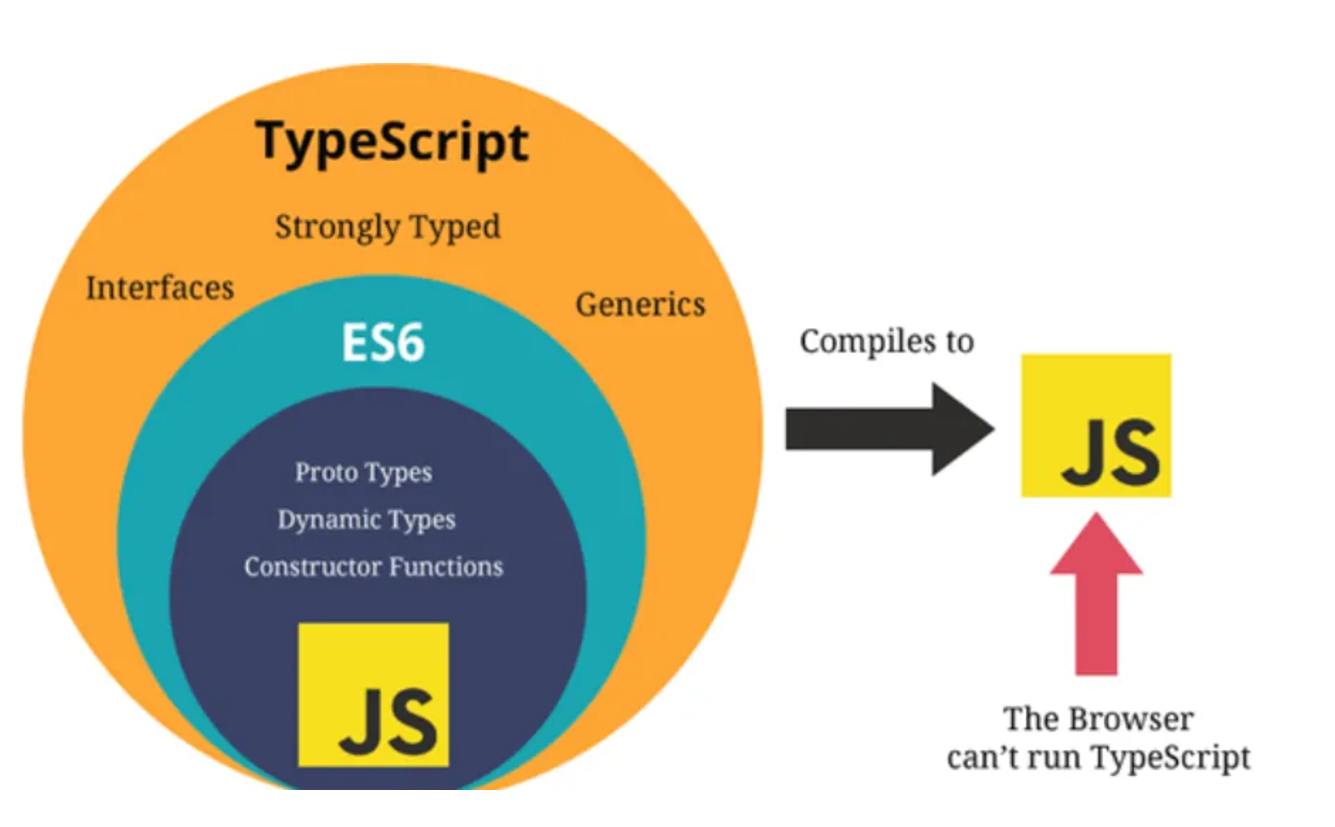
\includegraphics[scale=0.35]{tecnologie/javascript-typescript.png}
    \caption{Funzionalità di \textit{TypeScript} rispetto a \textit{JavaScript}}
    \cite{site:js-ts}
\end{figure}

\subsubsection{React}

\noindent Per la codifica del \gls{frontend} del progetto ho utilizzato \textit{React} con \textit{TypeScript}, per garantire una maggiore qualità e manutenibilità del codice.\\
Il \gls{frontend} di un’applicazione rappresenta la parte visibile ed interattiva con cui gli utenti interagiscono direttamente.
Include l’interfaccia utente, come pulsanti, menu, testi, immagini, e la logica che gestisce le loro interazioni.\\
Esso è responsabile dell’esperienza utente, garantendo che l’applicazione sia funzionale, veloce e visivamente accattivante su diversi dispositivi e \textit{browser}.\\

\noindent \textit{React} è una libreria \textit{JavaScript}, sviluppata da \textit{Meta}, progettata per la creazione di interfacce utente dinamiche e reattive. \\
Utilizzata nello sviluppo di applicazioni \textit{web} moderne, consente di costruire interfacce tramite un approccio basato su componenti,
ovvero blocchi modulari di codice che rappresentano singole parti dell’interfaccia, come pulsanti, schede o intere sezioni di una pagina.\\
Questi componenti sono codificati utilizzando \textit{file} con estensioni \textit{JavaScript} (\textit{JSX}) o \textit{TypeScript} (\textit{TSX}), permettendo di combinare logica e \textit{markup} in modo intuitivo.\\

\noindent \textit{React} è spesso utilizzato per creare \gls{spag}: applicazioni \textit{web} che caricano un'unica pagina \gls{html} ed aggiornano dinamicamente il contenuto in base all’interazione dell’utente, senza richiedere il caricamento completo della pagina.\\ 
Questo approccio garantisce un’esperienza utente fluida e veloce, simile a quella di un’applicazione \textit{desktop}, le \gls{spag} infatti gestiscono la navigazione attraverso il \textit{routing} \textit{client-side}.\\

\noindent L’integrazione di \textit{TypeScript} con \textit{React} è particolarmente utile in progetti complessi.
Grazie alla tipizzazione statica di \textit{TypeScript}, è possibile scrivere componenti più robusti e manutenibili, riducendo il rischio di errori e migliorando l’autocompletamento ed il \textit{refactoring},
garantendo che il comportamento dell’applicazione sia sempre prevedibile. \\

\subsubsection{Material UI}
Una libreria di componenti \textit{React} che implementa il \textit{Material Design}, uno stile di \textit{design} moderno sviluppato da \textit{Google}, progettato per garantire coerenza visiva, semplicità e accessibilità nelle interfacce utente.\\

\noindent Questa libreria fornisce un’ampia gamma di componenti predefiniti, come pulsanti, \textit{cards}, tabelle, e \textit{dialogs}, pronti all’uso e facilmente personalizzabili per adattarsi alle specifiche esigenze di un progetto. \\
Ogni componente è costruito per integrarsi perfettamente con l’ecosistema di \textit{React}, sfruttando appieno l’approccio basato su componenti e le funzionalità degli \textit{state} e dei \textit{props}.\\

\noindent Utilizzare questa libreria in un progetto \textit{React} semplifica la creazione di interfacce moderne, professionali e \textit{responsive}, riducendo significativamente il tempo necessario allo sviluppo, garantendo un’esperienza utente coerente e di alta qualità.\\

\subsubsection{Axios}

\textit{Axios} è una libreria \textit{JavaScript} progettata per semplificare la comunicazione tra il \gls{frontend} ed il \gls{backend} di un’applicazione, consentendo di effettuare richieste \gls{http} come \texttt{GET}, \texttt{POST}, \texttt{PUT} e \texttt{DELETE} in modo semplice e personalizzabile. \\
Supporta nativamente le \textit{Promises}, rendendo la gestione delle operazioni asincrone più chiara e leggibile, ed offre funzionalità avanzate come l’impostazione di intestazioni personalizzate, gestione automatica dei \textit{JSON},
\textit{timeout} configurabili e la possibilità di intercettare richieste e risposte per aggiungere logiche specifiche.\\

\noindent \gls{http} è uno \textit{standard} di comunicazione utilizzato su \textit{Internet} per il trasferimento di informazioni tra un \textit{client} (come un \textit{browser}) ed un \textit{server}.\\
Ogni interazione si basa su un modello di richiesta-risposta: il \textit{client} invia una richiesta al \textit{server} specificando l’azione desiderata (es. recuperare dati o inviarli), ed il \textit{server} risponde con le informazioni richieste o con un messaggio d’errore.\\

\noindent Il \gls{backend} di un’applicazione rappresenta la parte non visibile dall'utente, responsabile della logica di elaborazione dei dati, della gestione del \textit{database} e dell’esposizione delle \gls{api} necessarie per interagire con il \gls{frontend}.\\
Utilizzando \textit{Axios}, il \gls{frontend} può comunicare con il \gls{backend}, inviando dati come input dell’utente o recuperando contenuti dinamici, consentendo lo sviluppo di applicazioni \textit{web} moderne e interattive.\\

\noindent Le \gls{api} sono interfacce che consentono la comunicazione tra diverse applicazioni o componenti software, permettendo loro di scambiarsi dati e funzionalità. \\
Espongono un insieme di operazioni che possono essere invocate da altre applicazioni, nascondendo la complessità del sistema sottostante.\\
Ad esempio, possono essere utilizzate per recuperare dati da un \textit{database} o inviare informazioni ad un sistema di pagamento.\\

\noindent Le \gls{api} sono fondamentali per lo sviluppo di applicazioni moderne, poiché semplificano lo scambio di dati e permettono l’integrazione di diverse funzionalità, garantendo allo stesso tempo scalabilità e interoperabilità tra sistemi.

\subsubsection{Vite}

\textit{Vite} è uno strumento di sviluppo rapido e leggero che semplifica la configurazione e ottimizza il flusso di lavoro nel processo di sviluppo di applicazioni \textit{web}. \\
Utilizza \textit{ES Modules} per un caricamento veloce delle risorse ed una gestione ottimizzata dei moduli, riducendo i tempi di avvio e di aggiornamento durante lo sviluppo.\\

\noindent Quando utilizzato con \textit{React}, \textit{Vite} facilita la creazione di applicazioni configurando automaticamente il progetto, gestendo il \textit{bundling} ed il supporto per l'\textit{hot module replacement},
che permette di visualizzare istantaneamente le modifiche nel codice senza dover ricaricare la pagina, migliorando notevolmente l’esperienza di sviluppo.

\subsubsection{React-PDF}

\textit{React-PDF} è una libreria per il \textit{rendering} di documenti PDF direttamente all'interno di applicazioni \textit{React}. \\
Questa libreria consente di visualizzare \textit{file} PDF come componenti \textit{React}, rendendo possibile l'integrazione di documenti interattivi nelle pagine \textit{web} senza la necessità di \textit{software} esterni.\\

\noindent Con \textit{React-PDF}, è possibile caricare e mostrare file PDF, navigare tra le pagine, zoomare e persino aggiungere funzionalità interattive, come la gestione di eventi per rendere l’esperienza utente più dinamica. \\
Inoltre, la libreria offre il supporto per l’integrazione di funzionalità avanzate come la visualizzazione di PDF remoti o caricati dinamicamente.\\
\textit{React-PDF} è ideale per applicazioni che necessitano di visualizzare \textit{report}, documenti o qualsiasi altro tipo di contenuto PDF direttamente nel \textit{browser}.

\subsubsection{Styled Components}

\textit{Styled Components} è una libreria per \textit{React} che consente di scrivere stili \gls{css} direttamente all’interno dei componenti, utilizzando una sintassi che combina \gls{css} con \textit{JavaScript}.\\
Questa tecnica, nota come \textit{CSS-in-JS}, permette di definire e applicare stili personalizzati in modo modulare e dinamico per ciascun componente \textit{React}, migliorando la leggibilità e la manutenibilità del codice. 
Grazie a \textit{Styled Components}, è possibile creare componenti visivamente distinti, mantenendo il codice conciso e facilmente riutilizzabile.\\

\noindent La libreria si integra perfettamente con altre soluzioni di \textit{styling}, come \textit{Material-UI}, permettendo di personalizzare facilmente i componenti predefiniti di \textit{Material-UI} tramite stili aggiuntivi o sovrascritti. \\
In questo modo, si può beneficiare della potenza di \textit{Material-UI} per la creazione di interfacce utente moderne e responsive, mantenendo al contempo la flessibilità di \textit{Styled Components} per adattare l’aspetto visivo ai requisiti specifici del progetto. 

\subsubsection{Node.js}

\textit{Node.js} è un ambiente di \textit{runtime} per \textit{JavaScript} che consente di eseguire codice \textit{JavaScript} lato \textit{server}, utilizzando il motore V8 di \textit{Chrome}. \\
Questo permette di sviluppare applicazioni \textit{server-side}, sfruttando le stesse competenze di \textit{JavaScript} usate nel \gls{frontend}. \\
Il suo modello di programmazione asincrono e orientato agli eventi è ideale per gestire applicazioni scalabili e ad alte prestazioni, come \textit{server web}, \gls{apig} ed applicazioni in tempo reale.

\subsubsection{NestJS}

\noindent Per la codifica del \gls{backend} del progetto ho utilizzato \textit{NestJs}, un \textit{framework} \gls{backend} costruito sulla base di \textit{Node.js}, progettato per creare applicazioni \textit{server-side} moderne, scalabili ed efficienti.\\
Esso si distingue per il suo approccio modulare e l'adozione di \textit{TypeScript} come linguaggio principale, il che lo rende ideale per sviluppatori che cercano una struttura solida e una gestione ottimizzata del codice.\\
\textit{NestJS} utilizza le potenzialità di \textit{Node.js} per gestire applicazioni ad alte prestazioni e realizzare applicazioni \textit{server-side} complesse, come \gls{api-restful}, applicazioni in tempo reale e microservizi.\\

\noindent Grazie al suo supporto nativo per \textit{middleware}, guardie, filtri e \textit{interceptor}, \textit{NestJS} consente di implementare logiche complesse in modo chiaro e modulare.\\
Utilizza il modello asincrono e orientato agli eventi di \textit{Node.js} per gestire in modo efficiente le richieste e le operazioni contemporanee, garantendo prestazioni elevate anche in contesti con carichi pesanti.\\

\noindent Le \gls{api-restful} sono un insieme di convenzioni e \textit{best practices} per costruire interfacce di programmazione che permettano a \textit{client} e \textit{server} di comunicare attraverso il protocollo \gls{http}.\\
Esse si basano su risorse (ad esempio, dati o oggetti) che possono essere manipolate tramite operazioni standard di \gls{http}, come \textit{GET} (per recuperare dati), \textit{POST} (per creare nuovi dati), \textit{PUT} (per aggiornare dati esistenti) e \textit{DELETE} (per eliminare dati).\\
Grazie alla loro semplicità e scalabilità, le \gls{api-restful} sono ampiamente utilizzate nello sviluppo \textit{web} e \textit{mobile}.

\subsubsection{Zod}

\textit{Zod} è una libreria \textit{TypeScript} progettata per semplificare la validazione ed il \textit{parsing} dei dati. \\
Consente di definire \textit{schema} che specificano la forma ed i vincoli che i dati devono rispettare, permettendo di convalidare tipi di dati complessi come oggetti, stringhe, numeri, \textit{array}.\\
Il principale punto forza di \textit{Zod} risiede nella sua sintassi semplice e intuitiva, che permette di scrivere validazioni in modo dichiarativo e di catturare errori di tipo in fase di sviluppo, evitando \textit{bug} e problemi di coerenza nei dati.\\

\noindent Nel contesto dell'applicazione creata, ho utilizzato \textit{Zod} sia nel \gls{frontend} che nel \gls{backend} per garantire la correttezza dei dati.\\
Nel \gls{frontend}, \textit{Zod} viene impiegato per la validazione dei dati di \textit{login}, verificando che le credenziali inserite dall'utente siano nel formato corretto e rispettino determinati criteri (come la lunghezza minima della \textit{password} o la validità dell'indirizzo \textit{email}).\\
Questa validazione aiuta a migliorare l'esperienza utente e a ridurre gli errori lato \textit{client}.\\

\noindent Nel \gls{backend}, \textit{Zod} viene utilizzato per validare le richieste ricevute dal \gls{frontend}, garantendo che i dati abbiano la struttura corretta e soddisfino le condizioni necessarie prima di essere elaborati ulteriormente.\\
L'uso di \textit{Zod} nel \gls{backend} riduce la possibilità di errori nei dati in ingresso, contribuendo ad una gestione più sicura ed affidabile delle informazioni, migliorando anche la robustezza e la manutenibilità del codice.

\subsubsection{MongoDB}

Come \textit{database} ho utilizzato \textit{MongoDB}, un \textit{database NoSQL} altamente scalabile e flessibile, progettato per gestire dati sotto forma di documenti \textit{JSON-like}.\\
Questo tipo di \textit{database} è particolarmente indicato per applicazioni moderne che necessitano di una gestione efficiente di grandi volumi di dati non strutturati o semi-strutturati.\\
\textit{MongoDB} si distingue per la sua capacità di scalare orizzontalmente, ovvero di espandersi facilmente su più \textit{server}  per gestire carichi di lavoro elevati, senza compromettere le prestazioni. 
È anche molto versatile nell'integrazione con diverse tecnologie e ambienti, rendendolo una scelta popolare per progetti che richiedono flessibilità e rapidità nello sviluppo.\\

\noindent Una delle principali differenze tra un \textit{database SQL} (relazionale) e un \textit{database NoSQL} come \textit{MongoDB} riguarda la struttura dei dati.\\
Nei \textit{database SQL}, i dati sono organizzati in tabelle con righe e colonne, ed ogni riga deve rispettare uno schema fisso predefinito.\\
Ciò rende i \textit{database SQL} ideali per applicazioni con dati ben strutturati e con relazioni tra entità. \\
Tuttavia, questo approccio può risultare rigido quando si tratta di gestire dati complessi e non strutturati.\\

\noindent Al contrario, i \textit{database NoSQL} come \textit{MongoDB} non richiedono uno schema rigido. \\
I dati sono memorizzati in documenti che possono variare nel loro formato e struttura, il che consente una maggiore flessibilità.\\
Inoltre, i \textit{database NoSQL} sono progettati per supportare operazioni di lettura e scrittura rapide su grandi volumi di dati, ed offrono una maggiore scalabilità orizzontale,
il che significa che è più facile distribuire i dati su più \textit{server} per gestire l'aumento delle richieste senza compromettere le prestazioni.\\
Questo li rende particolarmente adatti per applicazioni \textit{web moderne} e scenari di microservizi.\\

\noindent Nella {\hyperref[fig:sql-nosql]{Figura 1.6}} è possibile vedere uno schema che mostra la differenza di struttura dei dati tra un \textit{database SQL} ed un \textit{database NoSQL}.

\begin{figure}[H]
    \label{fig:sql-nosql}
    \centering
    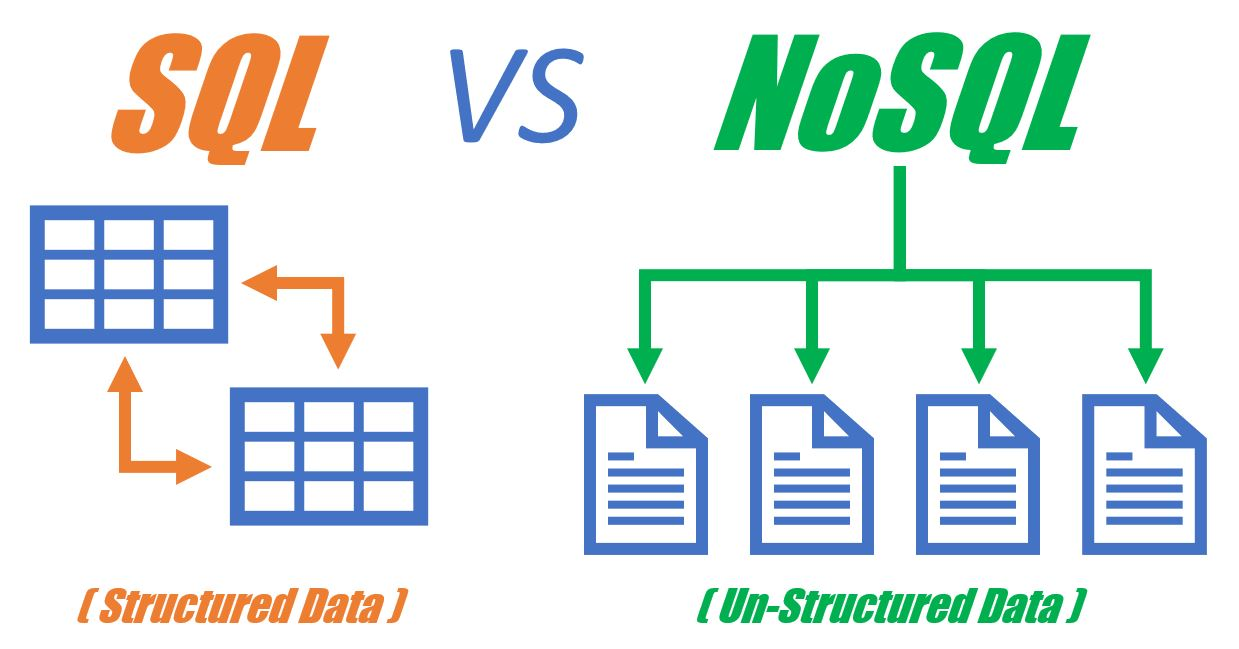
\includegraphics[scale=0.35]{tecnologie/sql-vs-nosql.jpg}
    \caption{Differente strutturazione dei dati in un \textit{database SQL} e in un \textit{database NoSQL}}
    \cite{site:sql-nosql}
\end{figure}

\pagebreak
\subsubsection{Mongoose}

\textit{Mongoose} è un \gls{odm} per \textit{Node.js}, progettato per semplificare l'interazione tra \textit{NestJS} e \textit{MongoDB}. \\
Un \gls{odm} è una libreria che fornisce un'interfaccia tra un \textit{database NoSQL} e il codice applicativo, consentendo agli sviluppatori di lavorare con oggetti \textit{JavaScript} anziché interagire direttamente con il database. \\
In altre parole, un \gls{odm} come \textit{Mongoose} trasforma i dati in formato \textit{JSON-like} di \textit{MongoDB} in oggetti \textit{JavaScript} più facilmente gestibili, semplificando operazioni come la creazione, la lettura, l'aggiornamento e la cancellazione.\\

\noindent In \textit{NestJS}, \textit{Mongoose} viene utilizzato per definire \textit{schema} di modelli, applicare validazioni e trasformazioni direttamente a livello di modello, e gestire \textit{middleware} personalizzati per ogni operazione.\\
Questo permette agli sviluppatori di definire strutture dati robuste, convalidare le informazioni in ingresso e uscita, e applicare logiche direttamente sulle entità. \\
\textit{Mongoose} supporta anche funzionalità avanzate come le \textit{query} complesse, il popolamento di documenti (per integrare dati da più collezioni) e la gestione delle relazioni tra documenti, rendendo la gestione dei dati in \textit{MongoDB} più intuitiva e scalabile all'interno di un'applicazione \textit{NestJS}.

\subsubsection{Puppeteer}

\textit{Puppeteer} è una libreria \textit{Node.js} che fornisce un'interfaccia di alto livello per controllare un \textit{browser} \gls{chromium} in modalità \textit{headless}, cioè senza interfaccia grafica, per automatizzare attività come il rendering di pagine \textit{web} e la generazione di \textit{file} PDF.\\
\textit{Chromium} è un \textit{browser open-source} sviluppato da \textit{Google}, che funge da base per browser come \textit{Google Chrome, Microsft Edge, ecc.}\\

\noindent Grazie a \textit{Puppeteer}, è possibile interagire programmaticamente con \textit{Chromium}, simulando l'esecuzione di \textit{script}, il caricamento di contenuti dinamici, l'interazione con il \textit{DOM}, e la creazione di documenti.\\

\noindent \textit{Puppeteer} è particolarmente utile per generare documenti PDF da template \textit{web}, mantenendo la formattazione, gli stili e i \textit{layout} originali, permettendo la personalizzazione di aspetti come margini, dimensioni della pagina e orientamento.\\
Questa libreria è stata impiegata nel progetto per generare \textit{file} PDF contenenti i dati dei progetti generati, assicurando la coerenza e l'alta qualità dei documenti prodotti, sia in termini di formato che di contenuti.

\subsubsection{HandleBars}

\textit{Handlebars} è una libreria \textit{JavaScript} che facilita la creazione e popolazione di \textit{template} \textit{HTML} con dati dinamici.\\
Grazie alla sua sintassi semplice ed estensibile, \textit{Handlebars} permette di separare la logica di presentazione dai dati, rendendo il codice più leggibile e manutenibile. \\
La libreria supporta l'uso di espressioni condizionali, cicli (\textit{loops}) ed \textit{helper} personalizzati, che permettono di manipolare e formattare i dati direttamente nel \textit{template}.\\

\pagebreak
\noindent Nel progetto, ho utilizzato \textit{Handlebars} per popolare un \textit{template} \textit{HTML} con i dati dinamici relativi ai progetti. \\
Successivamente, questo \textit{template} è stato passato a \textit{Puppeteer} per generare un \textit{file} PDF, mantenendo la formattazione e la struttura originale del \textit{template}.\\
Questo approccio consente di ottenere documenti PDF coerenti e ben strutturati, basati su dati personalizzati, con una gestione separata tra la logica e la presentazione.

\subsubsection{LangChain}

\textit{LangChain} è un \textit{framework} avanzato progettato per facilitare lo sviluppo di applicazioni che sfruttano i \gls{llm}. \\
Gli \gls{llm} sono modelli di intelligenza artificiale addestrati su grandi quantità di dati testuali per comprendere e generare linguaggio naturale. \\
Grazie alla loro dimensione e complessità, possono eseguire compiti come traduzione, riassunti, completamento di frasi, e risposte a domande in modo altamente sofisticato.\\
Per una spiegazione più dettagliata sugli \gls{llm} si rimanda alla {\hyperref[sez:llm]{sezione §2.3}}.\\

\noindent \textit{LangChain} semplifica l'interazione con modelli di linguaggio come quelli offerti da \gls{aws} \textit{Bedrock}, fornendo strumenti per gestire chiamate \gls{api}, orchestrare flussi di lavoro complessi, integrare memoria e combinare più modelli o fonti di dati in modo efficiente.\\
Nel progetto, ho utilizzato \textit{LangChain} insieme ad \gls{aws} \textit{Bedrock} per generare piani progettuali dettagliati. \\
Grazie alle sue capacità di orchestrazione, \textit{LangChain} ha permesso di ottimizzare i flussi di interazione tra i modelli di linguaggio e i dati, garantendo una gestione fluida delle richieste e delle risposte.\\

\noindent \textit{LangChain} include funzionalità avanzate come il \gls{prompt-engineering}, una disciplina dell'\gls{ai} che si occupa di progettare \textit{prompt} ottimizzati per ottenere risposte precise e di alta qualità dai modelli di linguaggio.\\
Il \gls{prompt-engineering} consiste nel definire accuratamente la struttura e il contenuto del \textit{prompt}, fornendo al modello un contesto chiaro e specifico per migliorare la pertinenza delle risposte.\\
Questa tecnica è fondamentale per massimizzare l’efficacia dei \textit{prompt} e personalizzare i risultati in base alle esigenze applicative, rendendo l’interazione con i modelli più mirata ed efficiente.\\

\noindent Un'altra funzionalità avanzata di \textit{LangChain} è la \gls{rag}\footcite{site:rag}. \\
Questa tecnica consente di migliorare le risposte dei modelli di linguaggio integrandole con una base di conoscenza esterna autorevole, al di fuori delle fonti di dati su cui i modelli sono stati addestrati.\\
La \gls{rag} permette di generare risposte più complesse e dettagliate, utilizzando documenti o \textit{database} specifici per il problema di riferimento.\\
Sebbene questa funzionalità non sia stata applicata direttamente nel progetto, rappresenta un'opzione potente per scenari che richiedono risposte altamente personalizzate e affidabili.\\
\textit{LangChain}, combinato con \gls{aws} \textit{Bedrock}, rappresenta quindi uno strumento versatile per creare applicazioni scalabili, sfruttando appieno le potenzialità degli \gls{llm} avanzati.

\noindent Nella {\hyperref[fig:langchain-usecases]{Figura 1.7}} è possibile vedere le principali funzionalità di \textit{LangChain}.


\begin{figure}[H]
    \label{fig:langchain-usecases}
    \centering
    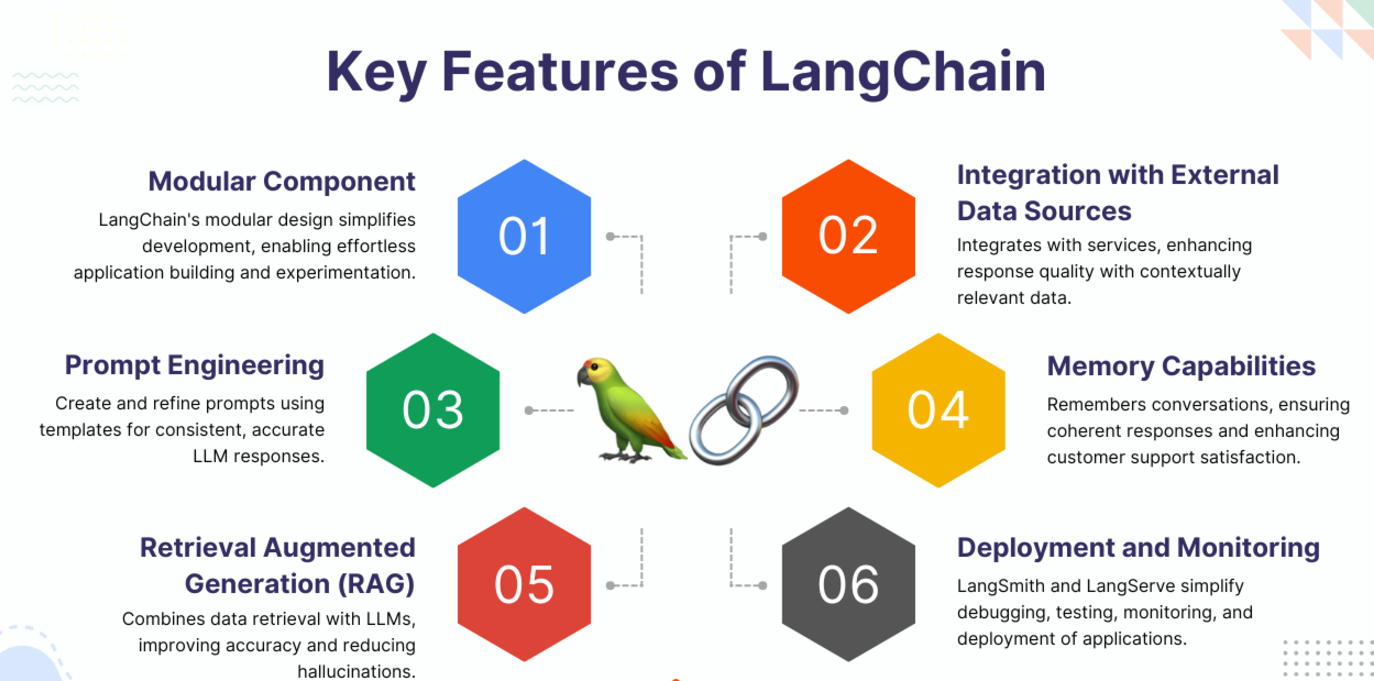
\includegraphics[scale=0.3]{tecnologie/langchain.png}
    \caption{Pricipali funzionalità di \textit{LangChain}}
    \cite{site:key-features-langchain}
\end{figure}

\subsubsection{AWS Amplify}

Una piattaforma completa per lo sviluppo di applicazioni \textit{web} e \textit{mobile} integrata con servizi \textit{cloud}.
\textit{AWS Amplify} fornisce strumenti per semplificare l’autenticazione degli utenti, la gestione delle \gls{api}, lo \textit{storage} di dati e l'\textit{hosting} delle applicazioni.\\

\noindent Consente agli sviluppatori di connettersi rapidamente con altri servizi \gls{aws}, supportando la creazione di applicazioni scalabili e moderne grazie a funzionalità come il monitoraggio in tempo reale, 
l’integrazione con \textit{framework} popolari ed il supporto per implementazioni \gls{ci/cd}.\\

\noindent \gls{ci/cd} sono pratiche di sviluppo \textit{software} che automatizzano l'integrazione continua del codice e il suo rilascio frequente. \\
Questi processi garantiscono maggiore efficienza, affidabilità e velocità nel ciclo di sviluppo.

\subsubsection{AWS Cognito}

Un servizio di gestione delle identità progettato per aggiungere funzionalità di autenticazione, registrazione e accesso federato alle applicazioni.\\
\textit{AWS Cognito} facilita la gestione degli utenti, offrendo opzioni di autenticazione tramite \gls{jwt}.\\

\noindent I \gls{jwt} sono \textit{token} standard utilizzati per trasferire in modo sicuro informazioni tra un \textit{client} ed un \textit{server}.\\
Essi contengono dati codificati (come l'identità dell'utente) e sono firmati digitalmente per garantire l'integrità e la sicurezza dei dati trasmessi.\\
Questi \textit{token} sono ideali per applicazioni \textit{web} moderne, poiché consentono una comunicazione senza necessità di sessioni persistenti sul \textit{server}, migliorando le prestazioni e la scalabilità.\\

\subsubsection{AWS Bedrock}

Un servizio di \gls{generative-ai} che permette agli sviluppatori di integrare modelli avanzati nelle proprie applicazioni senza dover possedere competenze specifiche in \gls{machine-learning}.\\

\noindent Il \gls{machine-learning} è una branca dell’intelligenza artificiale che si basa su algoritmi capaci di apprendere dai dati ed effettuare previsioni o prendere decisioni senza essere esplicitamente programmati.\\ 
La \gls{generative-ai}, invece, rappresenta una sottocategoria dell’intelligenza artificiale focalizzata sulla creazione di contenuti nuovi e originali, come testo, immagini, musica o codice,
basandosi su modelli pre-addestrati in grado di comprendere e replicare schemi presenti nei dati di addestramento.\\

\noindent Con \gls{aws} \textit{Bedrock}, gli sviluppatori possono sfruttare modelli pre-addestrati forniti da aziende leader del settore, con possibilità di personalizzazione per adattarli ai propri casi d’uso specifici.\\
Questo servizio è ideale per sviluppare soluzioni innovative come \textit{chatbot} avanzati, generazione di contenuti personalizzati, analisi approfondite di grandi volumi di dati e integrazione di funzionalità \gls{ai} scalabili nelle applicazioni.\\ 

\subsubsection{AWS S3 (\textit{Simple Storage Service})}

Un servizio di archiviazione \textit{cloud} progettato per memorizzare oggetti di qualsiasi dimensione con elevata scalabilità, disponibilità e sicurezza.\\
\textit{AWS S3} supporta il salvataggio di dati in forma di oggetti (\textit{blob}) organizzati in \textit{bucket}. È ideale per l’archiviazione e il recupero di file come immagini, video, documenti e \textit{backup}.\\

\noindent Include funzionalità avanzate come:
\begin{itemize}
    \item \textbf{Versionamento:} permette di gestire più versioni dello stesso \textit{file}, mantenendo traccia delle modifiche e consentendo di ripristinare versioni precedenti se necessario;
    \item \textbf{Controllo degli accessi:} per proteggere i dati e regolarne l'accesso tramite politiche di sicurezza granulari;
    \item \textbf{Integrazione con altri servizi \gls{aws}:} per analisi, distribuzione di contenuti o \gls{machine-learning}.
\end{itemize}

\noindent Nel progetto specifico, ho utilizzato \textit{AWS S3} per archiviare in modo sicuro i \textit{file} PDF generati dinamicamente.\\
Grazie alla funzionalità di versionamento di \textit{AWS S3}, ogni volta che un documento viene aggiornato o rigenerato, una nuova versione del \textit{file} viene automaticamente salvata, mantenendo le versioni precedenti accessibili.\\
Questo processo garantisce che le modifiche ai documenti siano tracciate e che si possieda una storicità completa dei \textit{file}, permettendo di ripristinare versioni precedenti in caso di necessità, il tutto senza compromettere l'affidabilità o la sicurezza dei dati.